\label{sec:event_selection}

\textbf{Z candidates} are defined as pairs of selected leptons (electrons or muons) with same flavour and opposite sign (SFOS).
They must satisfy $60 < m_{\Pl\Pl} < 120 \GeV$, where the Z candidate mass includes any selected FSR photons associated to its leptons.

\subsection{Four lepton channel}
In the 4\Pl channel, \textbf{ZZ candidates} are built from pairs of Z candidates with no lepton in common.
The first Z candidate $\PZ_1$ is chosen as the one with the reconstructed mass $m_{\Pl\Pl}$ closest to the nominal Z mass.
The second candidate is called $\PZ_2$.
The ZZ candidates are required to satisfy the following:
\begin{itemize}
\item Ghost removal: each of the four leptons must have $\DR > 0.02$ with any of the others.
  This requirement excludes ``ghost tracks'' made with a fraction of the hits of another lepton that produce an additional spurious lepton candidate.
\item Lepton \pt: the most energetic lepton must have $\pt^1 > 20 \GeV$ and the second most energetic $\pt^2 > 10 \GeV$,
  in order to ensure a high and constant trigger efficiency for all the selected events.
\item Low mass resonance suppression: all four opposite sign pairs, regardless of flavour, that can be built must satisfy $m_{\Pl\Pl} > 12 \GeV$.
  This cut suppresses pairs of leptons from cascade decays, which may have different flavour and are found to broadly peak at very low invariant masses.
  In this case, selected FSR photons are not used in computing $m_{\Pl\Pl}$, since a QCD-induced low mass di-lepton (\eg\ \JPsi) may have photons nearby (\eg from a \Pgpz).
\item Wrong pairing suppression: in the 4\Pe and 4\PGm channels,
  it is required that the alternative pairing of the four leptons does not result in
  an on-shell Z and a low mass $\Plp\Plm$ resonance with $m_{\Pl\Pl} < 12 \GeV$.
\item Four-lepton invariant mass: $m_{4\Pl} > 100 \GeV$.
\end{itemize}

\subsection{Three lepton channel}
In the 3\Pl channel the \PZ candidate is built first, using the pair of leptons with same flavour and opposite sign with the mass closest to the Z peak.
If no SFOS pair is found, the event is discarded.
the \PW is built with the third lepton and the MET. %% , which must be higher than 30 \GeV
The {\bf $\PW\PZ$ candidate} must then satisfy the same requirements of ghost removal and low mass resonance suppression imposed to the ZZ candidate in the 4\Pl channel.
Additionally:
\begin{itemize}
\item Lepton \pt: The two leptons from the \PZ boson must have $\pt^{\Pl_{Z,1}} > 25 \GeV$ and $\pt^{\Pl_{Z,2}} > 10 \GeV$,
  while the lepton in the \PW must have $\pt^{\Pl_{\PW}} > 25 \GeV$.
  As for the four lepton channel, this is to ensure high and constant trigger efficiency, by having at least two leptons ($\Pl_{Z,1}$ and $\Pl_\PW$)
  be above the threshold for the most energetic lepton of all the dilepton triggers,
  and that the third is above the less stringent threshold for the second lepton of such trigger paths.
\item \PZ mass: the \PZ boson mass must be within $15 \GeV$ from the \PZ mass peak.
\item Minimum MET: the missing energy must be $\MET > 30 \GeV$.
\item Three-lepton invariant mass: the invariant mass of the system of the three charged leptons is required to be $m_{3\Pl} > 100 \GeV$.
  This effectively suppresses contributions from $\PZ\PGg$ production where there is an asymmetric conversion of the photon that produces an electron.
\item b-veto: Events are rejected if there is at least one jet passing the medium b-tag threshold (see Section \ref{sec:jet_ID}).
  This is meant to suppress top quark backgrounds, like $\PQt\PAQt\PZ$ or $\PQt\PZ\PQq$ with a jet misidentified as photon.
\end{itemize}

\subsection{Two lepton channel}
The \PZ boson is build with the two leptons, which must be a SFOS pair.

The reconstruction of the hadronically decaying vector boson is intrinsically challenging,
since the large number of particles inside the jets degrades the resolution as compared to energetic and isolated leptons.
Furthermore, jet energy is sensitive to \pileup, both from charged and neutral particles, which must be accounted for.

When the vector boson is significantly boosted, the two quarks tend to be emitted with a small angle between them,
and thus the two jets have a small separation in \DR, causing them to overlap.
In this case, sometimes the clustering algorithm is not able to distinguish the two jets or cannot reconstruct them correctly.
Instead, it creates a single cluster, which often does not contain all the particles, and underestimates the energy of the jet.

For this kind of topology, one possible approach consists of running again the clustering algorithm with a larger value of the distance parameter D,
which is more likely to be able to include in an unique larger jet the particles coming from the quarks hadronization.
This creates a new set of jets which constitutes an alternative vision of the hadronic part of the event.

\begin{figure}
\centering
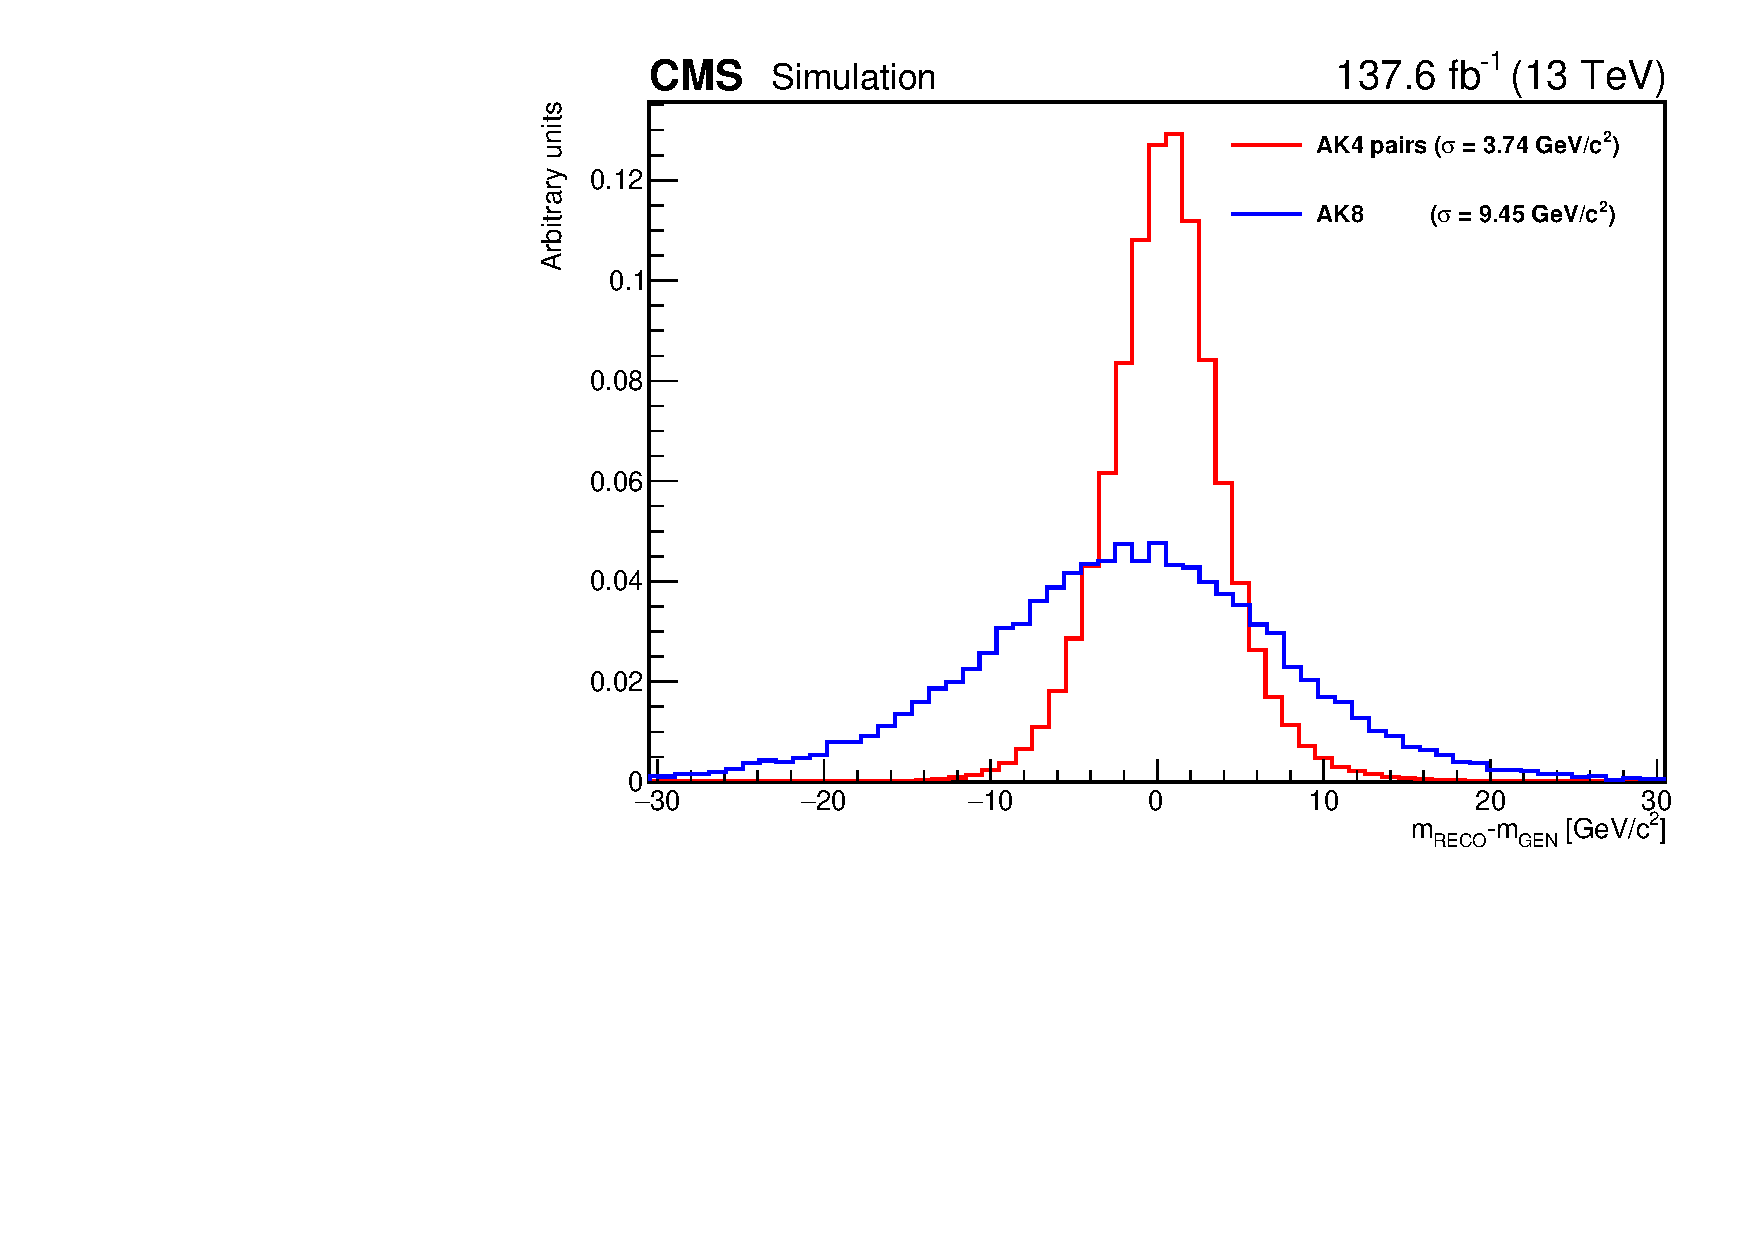
\includegraphics[width=0.5\textwidth]{AK_resolution_mass.pdf}
\caption{Resolution of the mass of reconstructed AK8 jets and pairs of AK4 jets, with respect to the generated objects.
The events correspond to the simulation of $\PZ\PZ\PGg \to 2\Pl\, 2j\, \PGg$ for the \RunII{} data taking period.
The two histograms are normalized to have unit area.}
\label{fig:AK_resolution_mass}
\end{figure}

From Figure~\ref{fig:AK_resolution_mass}, it is clear that pairs of AK4 jets are more precise in the reconstruction of the mass of the bosons.
This is caused by the larger number of \pileup{} particles included in a AK8 jet, which in turn require larger energy corrections or pruning, thus increasing the uncertainty.
Additionally the vector boson often does not have a very high transverse momentum,
so the resolved topology is more probable than the merged one.

\subsection{Photon selection}
\label{sec:evt_photon_selection}
The photon selection is common to the three channels.
Photons are required to have a transverse momentum $\pt^\PGg > 20 \GeV$
and be in the acceptance region of the ECAL, excluding the overlap region, $|\eta^\PGg| < 1.442$ OR $1.566 < |\eta^\PGg| < 2.4$.
The minimum separation between a photon and any of the leptons must be $\DR(\PGg, \Pl) > 0.5$.
Photons are required to pass the Conversion Safe Electron Veto.
%% and the Pixel Seed veto

Several photon IDs are compared in this analysis (see Section \ref{sec:photon_selection}):
the Loose working point of the cut-based ID
and the two working points \texttt{wp90} and \texttt{wp80} of the MVA-based ID.
In case there is more than one photon passing the requirements, the one with the highest \pt is selected.

For the results on the significance of triboson production, the cut designed to suppress FSR contributions
described in Section~\ref{sec:FSR_cut} is also applied.
